\documentclass[journal,12pt,onecolumn]{IEEEtran}
\usepackage{graphicx, float}
\graphicspath{{Figs/}}
\usepackage{multicol}
\usepackage{parskip}
\usepackage{titlesec}
\usepackage{color}
\usepackage{enumitem}
\usepackage{amsmath,amssymb,amsfonts,amsthm}
\usepackage{array}
\usepackage{booktabs}
\usepackage[table]{xcolor}
\usepackage{longtable}
\usepackage{gensymb}
\usepackage{cite}
\usepackage{algorithmic}
\usepackage{textcomp}
\usepackage{txfonts}
\usepackage{listings}
\usepackage{mathtools}
\usepackage{comment}
\usepackage{tkz-euclide}
\usepackage[breaklinks=true]{hyperref}
\usepackage{gvv}
\usepackage[utf8]{inputenc}
\usetikzlibrary{arrows.meta, positioning}
\usepackage{xparse}
\usepackage{calc}
\usepackage{multirow}
\usepackage{hhline}
\usepackage{ifthen}
\usepackage{lscape}
\usepackage{tabularx}

\begin{document}

\title{
ASSIGNMENT 1: GATE 2011 \\
BT: BIOTECHNOLOGY ENGINEERING}
\author{AI25BTECH11025-R Nikhil}
\maketitle
\renewcommand{\thefigure}{\theenumi}
\renewcommand{\thetable}{\theenumi}

\begin{center}
    \textbf{2011} \hfill \textbf{BT : BIOTECHNOLOGY} \hfill \textbf{BT} \\[6pt]
    \textit{Duration: Three Hours} \hfill \textit{Maximum Marks: 100}
\end{center}


\noindent \textbf{Read the following instructions carefully.}
\begin{enumerate}
    \item Write your name and registration number in the space provided at the bottom of this page.
    \item Take out the Optical Response Sheet (ORS) from this Question Booklet \textbf{without breaking the seal}.
    \item Do not open the seal of the Question Booklet until you are asked to do so by the invigilator.
    \item Write your registration number, your name and name of the examination centre at the specified locations on the right half of the ORS. Also, using HB pencil, darken the appropriate bubble under each digit of your registration number and the letters corresponding to your test paper code (BT).
    \item This Question Booklet contains \textbf{16 pages} including blank pages for rough work. After opening the seal at the specified time, please check all pages and report discrepancy, if any.
    \item There are a total of 65 questions carrying 100 marks. All these questions are of objective type. Questions must be answered on the left hand side of the ORS by darkening the appropriate bubble (marked A, B, C, D) using HB pencil against the question number. For \textbf{each question darken the bubble of the correct answer}. In case you wish to change an answer, erase the old answer completely. More than one answer bubbled against a question will be treated as an incorrect response.
    \item Questions Q.1 – Q.25 carry 1-mark each, and questions Q.26 – Q.55 carry 2-marks each.
    \item Questions Q.48 – Q.51 (2 pairs) are common data questions and question pairs (Q.52, Q.53) and (Q.54, Q.55) are linked answer questions. The answer to the second question of the linked answer questions depends on the answer to the first question of the pair. If the first question in the linked pair is wrongly answered or is unattempted, then the answer to the second question in the pair will not be evaluated.
    \item Questions Q.56 – Q.65 belong to General Aptitude (GA). Questions Q.56 – Q.60 carry 1-mark each, and questions Q.61 – Q.65 carry 2-marks each. The GA questions begin on a fresh page starting from page 12.
    \item Unattempted questions will result in zero mark and wrong answers will result in \textbf{NEGATIVE marks}. For Q.1 – Q.25 and Q.56 – Q.60, $\tfrac{1}{3}$ mark will be deducted for each wrong answer. For Q.26 – Q.51 and Q.61 – Q.65, $\tfrac{2}{3}$ mark will be deducted for each wrong answer. The question pairs (Q.52, Q.53) and (Q.54, Q.55) are questions with linked answers. There will be negative marks only for wrong answer to the first question of the linked answer question pair, i.e. for Q.52 and Q.54, $\tfrac{2}{3}$ mark will be deducted for each wrong answer. There is no negative marking for Q.53 and Q.55.
    \item Calculator is allowed whereas charts, graph sheets or tables are \textbf{NOT} allowed in the examination hall.
    \item Rough work can be done on the question paper itself. Additionally, blank pages are provided at the end of the question paper for rough work.
\end{enumerate}

\vfill

\noindent\begin{tabular}{|p{7cm}|}
\hline
Name \\[1.5cm] \\
\hline
Registration Number \hfill \textbf{BT} \\[1.5cm] \\
\hline
\end{tabular}

\section*{Q.1 – Q.25 carry one mark each}

\begin{enumerate}

    \item Embryonic stem cells are derived from
    \begin{multicols}{2}
    \begin{enumerate}
        \item fertilized embryo
        \item unfertilized embryo
        \item sperm
        \item kidney
    \end{enumerate}
    \end{multicols} \hfill(GATE BT 2011)

    \item Members of the antibody protein family that have common structural features are collectively known as
    \begin{multicols}{2}
    \begin{enumerate}
        \item haptens
        \item allergens
        \item antigens
        \item immunoglobulins
    \end{enumerate}
    \end{multicols} \hfill(GATE BT 2011)

    \item Apoptosis is characterized by
    \begin{multicols}{2}
    \begin{enumerate}
        \item necrosis
        \item programmed cell death
        \item membrane leaky syndrome
        \item cell cycle arrest process
    \end{enumerate}
    \end{multicols} \hfill(GATE BT 2011)

    \item Yeast artificial chromosomes (YAC’s) are used for cloning
    \begin{multicols}{2}
    \begin{enumerate}
        \item large segments of DNA
        \item mRNA
        \item bacterial DNA
        \item yeast DNA
    \end{enumerate}
    \end{multicols} \hfill(GATE BT 2011)

    \item The product commercially produced by animal cell culture is
    \begin{multicols}{2}
    \begin{enumerate}
        \item insulin
        \item tissue plasminogen activator
        \item interferon
        \item hepatitis B vaccine
    \end{enumerate}
    \end{multicols} \hfill(GATE BT 2011)

    \item An alternative to glycolysis pathway is
    \begin{multicols}{2}
    \begin{enumerate}
        \item glyoxylate pathway
        \item pentose phosphate pathway
        \item citric acid cycle
        \item gluconeogenesis
    \end{enumerate}
    \end{multicols} \hfill(GATE BT 2011)

    \item A cell in G$_1$ of interphase has 12 chromosomes. How many chromatids will be found per cell during metaphase II of meiosis?
    \begin{multicols}{2}
    \begin{enumerate}
        \item 6
        \item 12
        \item 18
        \item 24
    \end{enumerate}
    \end{multicols} \hfill(GATE BT 2011)

    \item Diploid \textit{Drosophila} has eight chromosomes. Which one of the following terms should \textbf{NOT} be used to describe \textit{Drosophila} with sixteen numbers of chromosomes?
    \begin{multicols}{2}
    \begin{enumerate}
        \item Polyploid
        \item Aneuploid
        \item Euploid
        \item Tetraploid
    \end{enumerate}
    \end{multicols} \hfill(GATE BT 2011)

    \item Hydrated synthetic seeds which are produced by ion exchange reaction involve mixing the somatic embryos in a solution of
    \begin{enumerate}
        \item sodium alginate and dropping it in a solution of calcium nitrate
        \item calcium alginate and dropping it in a solution of sodium nitrate
        \item calcium alginate and dropping it in a solution of ammonium nitrate
        \item mannitol and dropping it in a solution of sodium nitrate
    \end{enumerate}
    \hfill(GATE BT 2011)
    
\item Shoot organogenesis by tissue culture results into
    \begin{enumerate}
        \item a bipolar structure that has no vascular connection with the explant
        \item a monopolar structure that has a strong connection with the pre-existing vascular tissue of the explant
        \item a monopolar structure that has no vascular connection with the explant
        \item a bipolar structure that has a strong connection with the pre-existing vascular tissue of the explant
    \end{enumerate}
     \hfill(GATE BT 2011)

\item ‘Hairy roots’ induced \textit{in vitro} by the infection of \textit{Agrobacterium rhizogenes}, are characterized by 

    P. a high degree of lateral branching  \\
    Q. genetic instability of culture  \\
    R. an absence of geotropism\\
    S. poor biomass production  

    \begin{multicols}{2}
    \begin{enumerate}
        \item P and R only
        \item P and Q only
        \item Q and R only
        \item R and S only
    \end{enumerate}
    \end{multicols} \hfill(GATE BT 2011)

    \item In balanced growth phase of a cell 

    P. all components of a cell grow at the same rate 
    
    Q. specific growth determined by cell number or cell mass would be the same  
    
    R. the growth rate is independent of substrate concentration  
    
    S. the growth rate decreases with decreasing substrate concentration  

    \begin{multicols}{2}
    \begin{enumerate}
        \item P, Q and S only
        \item Q, R and S only
        \item P, Q and R only
        \item P only
    \end{enumerate}
    \end{multicols} \hfill(GATE BT 2011)

    \item In N-linked glycosylation, the oligosaccharide chain is attached to protein by
    \begin{multicols}{2}
    \begin{enumerate}
        \item asparagine
        \item arginine
        \item serine
        \item threonine
    \end{enumerate}
    \end{multicols} \hfill(GATE BT 2011)

    \item Restriction endonucleases which recognize and cut same recognition sequences are known as
    \begin{multicols}{2}
    \begin{enumerate}
        \item isoschizomers
        \item isozymes
        \item isoaccepting endonucleases
        \item abzymes
    \end{enumerate}
    \end{multicols} \hfill(GATE BT 2011)

    \item Substrate consumption in lag phase of microbial growth is primarily used for  

    P. turn over of the cell material 
    
    Q. maintenance of intracellular pH 
    
    R. motility  
    
    S. increase in cell number 

    \begin{multicols}{2}
    \begin{enumerate}
        \item P, Q and S only
        \item Q, R and S only
        \item P, Q and R only
        \item S only
    \end{enumerate}
    \end{multicols} \hfill(GATE BT 2011)
    
\item Wash out (as defined by $D = D_{\text{max}}$) of a continuous stirred tank fermenter is characterized by \\
(X = biomass, S = substrate concentration in bioreactor, $S_0$ = substrate concentration in feed, P = product concentration in bioreactor)  
\begin{multicols}{2}
\begin{enumerate}
\item $X = 0, S = 0, P = 0$  
\item $X = 0, S = S_0, P = 0$  
\item $X = 0, S < S_0, P = 0$  
\item $X < 0, S < S_0, P < 0$  
\end{enumerate}
\end{multicols} \hfill(GATE BT 2011)

\item The study of evolutionary relationships is known as  
\begin{multicols}{2}
\begin{enumerate}
\item genomics  
\item proteomics  
\item phylogenetics  
\item genetics  
\end{enumerate}
\end{multicols} \hfill(GATE BT 2011)

\item The lipopolysaccharides present in bacterial cell wall has lipid A which is connected to  
\begin{enumerate}
\item O-polysaccharide  
\item core polysaccharide  
\item both O-polysaccharide and core polysaccharide  
\item rhamnose-mannose disaccharide  
\end{enumerate}
\hfill(GATE BT 2011)

\item Molecular chaperones are class of proteins that facilitate  
\begin{enumerate}
\item the proper folding of newly synthesized proteins  
\item unfolding of newly synthesized proteins  
\item degradation of newly synthesized proteins  
\item targeting of newly synthesized proteins  
\end{enumerate}
\hfill(GATE BT 2011)


\item Gas vacuoles are present in  
\begin{enumerate}
\item \textit{Anabaena flos-aquae}  
\item \textit{Bacillus subtilis}  
\item \textit{Acathamoeba nifrigiscens}  
\item \textit{Mycobacterium tuberculosis}  
\end{enumerate}
\hfill(GATE BT 2011)

\item In ABO blood group system, antigenic determinants are  
\begin{multicols}{2}
\begin{enumerate}
\item nucleic acid  
\item carbohydrate  
\item lipid  
\item protein  
\end{enumerate}
\end{multicols} \hfill(GATE BT 2011)

\item The most widely used program for multiple sequence alignment is  
\begin{multicols}{2}
\begin{enumerate}
\item BLAST  
\item FASTA  
\item CLUSTAL  
\item Chime  
\end{enumerate}
\end{multicols} \hfill(GATE BT 2011)

\item Diphtheria toxin, tetracycline and streptomycin inhibit  
\begin{multicols}{2}
\begin{enumerate}
\item DNA repair  
\item DNA replication  
\item transcription  
\item translation  
\end{enumerate}
\end{multicols} \hfill(GATE BT 2011)

\item The polymorphic domains for Class II MHC proteins are  
\begin{multicols}{2}
\begin{enumerate}
\item $\alpha_1$ and $\beta_1$ domains only  
\item $\beta_1$ and $\beta_2$ domains only  
\item $\alpha_1$ and $\beta_2$ domains only  
\item $\alpha_2$ and $\beta_1$ domains only  
\end{enumerate}
\end{multicols} \hfill(GATE BT 2011)

\item The protein in eukaryotes which is subjected to degradation undergoes  
\begin{multicols}{2}
\begin{enumerate}
\item phosphorylation  
\item carboxylation  
\item ubiquitination  
\item methylation  
\end{enumerate}
\end{multicols} \hfill(GATE BT 2011)

\item Match the viruses in Group I with their host cell receptors in Group II.  
\begin{multicols}{2}
  Group I
  \begin{enumerate}
    \item[P.] Hepatitis A virus  
    \item[Q.] Human immunodeficiency virus  
    \item[R.] Rabies virus  
    \item[S.] Herpes simplex virus type I  
  \end{enumerate}


  Group II
  \begin{enumerate}
    \item[1.] Heparan sulphate  
    \item[2.] Acetylcholine receptor  
    \item[3.] CD4 protein  
    \item[4.] Alpha-2 macroglobulin  
  \end{enumerate}
\end{multicols} 

  \begin{multicols}{2}
  \begin{enumerate}
    \item P-1, Q-3, R-2, S-4  
    \item P-3, Q-4, R-1, S-2  
    \item P-4, Q-3, R-2, S-1  
    \item P-2, Q-3, R-1, S-4  
  \end{enumerate}
  \end{multicols} \hfill(GATE BT 2011)


  \item Match the microbial growth characteristics in \textbf{Group I} 
  with the corresponding features in \textbf{Group II}. 

  \begin{table}[H]
  \centering
\begin{tabular}{cc}
    \textbf{Group I}  & \textbf{Group II}  \\
    P. Growth associated product formation & 1. Specific growth rate decreases with increasing product concentration \\ 
    Q. Non growth associated product formation & 2. Specific product formation rate is constant \\ 
    R. Product inhibition & 3. Specific product formation rate is proportional to specific growth rate \\ 
    S. Substrate inhibition & 4. Specific growth rate decreases with increasing substrate concentration \\
  \end{tabular}
  \end{table}

  \begin{multicols}{2}
  \begin{enumerate}
    \item $P \to 1,\; Q \to 2,\; R \to 4,\; S \to 3$
    \item $P \to 3,\; Q \to 2,\; R \to 1,\; S \to 4$
    \item $P \to 2,\; Q \to 1,\; R \to 3,\; S \to 4$
    \item $P \to 2,\; Q \to 3,\; R \to 4,\; S \to 1$
  \end{enumerate}
  \end{multicols}\hfill(GATE BT 2011)


  \item Match the items in \textbf{Group I} with \textbf{Group II}.
  
  \begin{table}[H]
  \centering
  \begin{tabular}{cc}
    \textbf{Group I}  & \textbf{Group II}  \\ 
    P. Circular dichroism & 1. Concentration \\ 
    Q. X-ray crystallography & 2. Sedimentation coefficient \\ 
    R. Freeze-drying & 3. Secondary structure determination \\ 
    S. Ultracentrifugation & 4. Tertiary structure determination \\
  \end{tabular}
  \end{table}

  \begin{multicols}{2}
  \begin{enumerate}
    \item[(A)] $P \to 4,\; Q \to 1,\; R \to 2,\; S \to 3$
    \item[(B)] $P \to 1,\; Q \to 4,\; R \to 3,\; S \to 2$
    \item[(C)] $P \to 2,\; Q \to 3,\; R \to 4,\; S \to 1$
    \item[(D)] $P \to 3,\; Q \to 4,\; R \to 1,\; S \to 2$
  \end{enumerate}
  \end{multicols}
  \hfill(GATE BT 2011)
  
\item Match the products in Group I with their respective organisms in Group II.  

\begin{table}[H]
  \begin{tabular}{p{4cm} p{6cm}}
    \textbf{Group I}    & \textbf{Group II} \\
    P. Glycerol         & 1. Corynebacterium glutamicum \\
    Q. Glutamic acid    & 2. Alcaligenes faecalis \\
    R. Curdlan          & 3. Dunaliella salina \\
    S. Actinomycin B    & 4. Streptomyces nodosus \\
  \end{tabular}
  \end{table}
  
  \begin{multicols}{2}
  \begin{enumerate}
    \item P-2, Q-1, R-3, S-4  
    \item P-4, Q-2, R-1, S-3  
    \item P-3, Q-1, R-2, S-4  
    \item P-2, Q-1, R-4, S-3  
  \end{enumerate}
  \end{multicols} \hfill(GATE BT 2011)

\item Determine the correctness or otherwise of the following Assertion (a) and the Reason (r).  

\textbf{Assertion}: $I_gM$ is found in serum as a pentameric protein consisting of fiv $I_gM$ monomers.  

\textbf{Reason}: The pentameric form of $I_gM$ is due to cross-linking of $I_gM$ monomers via peptide bond.  

\begin{enumerate}
  \item Both (a) and (r) are true and (r) is the correct reason for (a)  
  \item Both (a) and (r) are true but (r) is not the correct reason for (a)  
  \item (a) is true but (r) is false  
  \item (a) is false but (r) is true  
\end{enumerate}
\hfill(GATE BT 2011)

\item Determine the correctness or otherwise of the following Assertion (a) and the Reason (r).  

\textbf{Assertion}:   N-methyl-N'-nitro-N-nitrosoguanidine (NTG) is an effective chemical mutagen.  

\textbf{Reason}:   Mutations induced by NTG mainly are the GC $\rightarrow$ AT transitions.  

\begin{enumerate}
  \item Both (a) and (r) are true and (r) is the correct reason for (a)  
  \item Both (a) and (r) are true but (r) is not the correct reason for (a)  
  \item (a) is true but (r) is false  
  \item (a) is false but (r) is true  
\end{enumerate}
\hfill(GATE BT 2011)



\item Determine the correctness of the following statements  

I. Enhancer sequences are those DNA sequences that are involved in increasing the rate of DNA replication. \\ 
II. Enhancer sequences work by binding with eukaryotic gene activator factors.  

\begin{multicols}{2}
\begin{enumerate}
  \item Only I is true  
  \item Only II is true  
  \item Both I and II are true  
  \item Both I and II are false  
\end{enumerate}
\end{multicols} \hfill(GATE BT 2011)

    \item In a well aerated and agitated microbial culture, the `supply' of oxygen is equal to 
    `demand' (uptake) of the growing culture. The $K_La$ for such a system will be 
    \\
    ($K_La =$ volumetric mass transfer coefficient, $C^* =$ dissolved oxygen concentration in liquid 
    in equilibrium with gaseous oxygen, $C =$ instantaneous value of dissolved oxygen concentration, 
    $r =$ specific oxygen uptake rate per unit weight of cells, $X =$ dry weight of the cells per unit volume).
    
    \begin{multicols}{2}
    \begin{enumerate}
        \item $(rX) / (C^* - C)$
        \item $r / \{ X (C^* - C) \}$
        \item $(C^* - C) / (rX)$
        \item $X / \{ r (C^* - C) \}$
    \end{enumerate}
    \end{multicols} \hfill(GATE BT 2011)
  
  \item Structured William’s model
  \begin{enumerate}
    \item[P.] can describe the changes in intracellular components of the cell during growth
    \item[Q.] can not describe the death phase of the cells
    \item[R.] can describe the variation of size of cells in the different phases of growth
    \item[S.] can not describe the lag period of growth
  \end{enumerate}

  Which one of the following is \textbf{CORRECT}?
  \begin{multicols}{2}
    \begin{enumerate}
      \item P, Q and S only
      \item P, Q and R only
      \item Q, R and S only
      \item P, R and S only
    \end{enumerate}
  \end{multicols} \hfill(GATE BT 2011)

  % Q35
  \item Match items in Group I with Group II.

  \begin{table}[H]
  \centering
  \begin{tabular}{cc}

    \textbf{Group I} & \textbf{Group II} \\
    P. Glycolytic pathway & 1. Chloroplast \\
    Q. Eukaryotic oxidative metabolism & 2. Glyoxysomes \\
    R. Glyoxylate cycle & 3. Mitochondria \\
    S. Calvin cycle & 4. Cytosol \\

  \end{tabular}
  \end{table}

  \begin{multicols}{2}
    \begin{enumerate}
      \item P-1, Q-2, R-3, S-4
      \item P-2, Q-3, R-4, S-1
      \item P-4, Q-3, R-2, S-1
      \item P-3, Q-4, R-1, S-2
    \end{enumerate}
  \end{multicols} \hfill(GATE BT 2011)

  % Q36
  \item Match items in Group I with Group II.

  \begin{table}[H]
  \centering
  \begin{tabular}{cc}
    \textbf{Group I} & \textbf{Group II} \\
    P. Alzheimer’s disease & 1. H1N1 \\
    Q. Mad cow disease & 2. Hemoglobin \\
    R. Sickle cell anaemia & 3. Prions \\
    S. Swine flu & 4. Amyloid \\
  \end{tabular}
  \end{table}

  \begin{multicols}{2}
    \begin{enumerate}
      \item P-4, Q-3, R-2, S-1
      \item P-3, Q-4, R-1, S-2
      \item P-2, Q-1, R-4, S-3
      \item P-1, Q-2, R-3, S-4
    \end{enumerate}
  \end{multicols} \hfill(GATE BT 2011)

  % Q37
  \item Determine the correctness or otherwise of the following Assertion (a) and the Reason (r) \\
  \textbf{Assertion}: The elucidation of ribosome structure helps in the development of new generation drugs. \\
  \textbf{Reason}: The high resolution of macromolecular structure has enabled in structure-based drug design. 

    \begin{enumerate}
      \item Both (a) and (r) are true and (r) is the correct reason for (a)
      \item Both (a) and (r) are true but (r) is not the correct reason for (a)
      \item(a) is true but (r) is false
      \item (a) is false but (r) is true
    \end{enumerate}
    \hfill(GATE BT 2011)

  % Q38
  \item Determine the correctness or otherwise of the following Assertion (a) and the Reason (r) \\
  \textbf{Assertion}: A very low amount of inhibitor can act as an activator for allosteric enzymes. \\
  \textbf{Reason}: Allosteric enzymes follow Michaelis--Menten kinetics. 

  
    \begin{enumerate}
      \item Both (a) and (r) are true and (r) is the correct reason for (a)
      \item Both (a) and (r) are true but (r) is not the correct reason for (a)
      \item (a) is true but (r) is false
      \item (a) is false but (r) is true
    \end{enumerate}
    \hfill(GATE BT 2011)
  

  % Q39
  \item Match the terms in Group I with their associated functions in Group II. 

  \begin{table}[H]
  \centering
  \begin{tabular}{c c}
    \textbf{Group I} & \textbf{Group II} \\
    P. Shine–Dalgarno sequences & 1. Aminoacylation of tRNA \\
    Q. Leucine zipper & 2. Gene silencing \\
    R. Aminoacyl tRNA synthetase & 3. Ribosome binding and facilitation of initiation \\
    S. RNA interference (RNAi) & 4. Transcription factors \\
  \end{tabular}
  \end{table}

  \begin{multicols}{2}
    \begin{enumerate}
      \item P-3, Q-4, R-1, S-2
      \item P-4, Q-3, R-2, S-1
      \item P-2, Q-3, R-1, S-4
      \item P-3, Q-2, R-4, S-1
    \end{enumerate}
  \end{multicols} \hfill(GATE BT 2011)

  % Q40
  \item Protein–protein interactions are studied by
  \begin{enumerate}
    \item[P.] DNA foot printing
    \item[Q.] Yeast two hybrid system
    \item[R.] Ligation chain reaction
    \item[S.] Mass spectrometry
  \end{enumerate}

  \begin{multicols}{2}
    \begin{enumerate}
      \item P and S only
      \item Q and S only
      \item P and Q only
      \item Q and R only
    \end{enumerate}
  \end{multicols} \hfill(GATE BT 2011)

  % Q41
  \item Determine the correctness or otherwise of the following Assertion (a) and the Reason (r) \\
  \textbf{Assertion}: Isopropylthiogalactoside (IPTG) is a gratuitous inducer of lactose operon. \\
  \textbf{Reason}: Gratuitous inducers are chemical analogues which behave like natural inducer but they do not serve as substrate for the enzymes that are subsequently induced.

    \begin{enumerate}
      \item Both (a) and (r) are true and (r) is the correct reason for (a)
      \item Both (a) and (r) are true but (r) is not the correct reason for (a)
      \item (a) is true but (r) is false
      \item (a) is false but (r) is true
    \end{enumerate}
    \hfill(GATE BT 2011)

  % Q42
  \item Determine the correctness or otherwise of the following Assertion (a) and the Reason (r) \\
  \textbf{Assertion}: In synchronous culture, majority of the cells move to next phase of the cell cycle simultaneously. \\
  \textbf{Reason}: Synchronous culture could be obtained by starving cells for essential nutrient components.

    \begin{enumerate}
      \item Both (a) and (r) are true and (r) is the correct reason for (a)
      \item Both (a) and (r) are true but (r) is not the correct reason for (a)
      \item (a) is true but (r) is false
      \item (a) is false but (r) is true
    \end{enumerate}
 \hfill(GATE BT 2011)
    

  % Q43
  \item Which of the following characteristics with respect to bacterial DNA polymerase III are \textbf{TRUE}?
  \begin{enumerate}
    \item[P.] Initiation of chain synthesis
    \item[Q.] $5' \to 3'$ polymerization
    \item[R.] $3' \to 5'$ exonuclease activity
    \item[S.] $5' \to 3'$ exonuclease activity
  \end{enumerate}

  \begin{multicols}{2}
    \begin{enumerate}
      \item P and Q only
      \item Q and R only
      \item Q and S only
      \item P and S only
    \end{enumerate}
  \end{multicols} \hfill(GATE BT 2011)

  % Q44
  \item Maximum specific growth rate $(\mu_{\max})$ of a microorganism is calculated by taking the 
  $\ln = \log_e X, \; X =$ biomass, $t =$ time
    \begin{enumerate}
      \item slope of $\ln X$ vs $t$ of the growth cycle
      \item slope of $\ln X$ vs $t$ during the exponential growth phase
      \item slope of $X$ vs $t$
      \item slope of $X$ vs $t$ during the exponential phase of growth
    \end{enumerate}
    \hfill(GATE BT 2011)

  % Q45
  \item Identify the \textbf{CORRECT} statements
  \begin{enumerate}
    \item[P.] $5'$ and $3'$ ends of the transcripts can be mapped by utilizing polymerase chain reaction
    \item[Q.] S$_1$ nuclease can cleave the DNA strand of a DNA-RNA hybrid
    \item[R.] T$_4$ polynucleotide kinase is used for labeling $3'$ end of DNA
    \item[S.] Baculovirus \textit{(Autographa californica)} can be used as an insect expression vector
  \end{enumerate}

  \begin{multicols}{2}
    \begin{enumerate}
      \item P and Q only
      \item R and S only
      \item P and S only
      \item Q and R only
    \end{enumerate}
  \end{multicols} \hfill(GATE BT 2011)

  % Q46
  \item Value of the determinant mentioned below is
  \[
  \begin{vmatrix}
  1 & 0 & -1 & 0 \\
  4 & 7 & 0 & 2 \\
  1 & 1 & -1 & 1 \\
  2 & 0 & 2 & 1
  \end{vmatrix}
  \]

   \begin{multicols}{4}   
    \begin{enumerate}
      \item 24
      \item -30
      \item -24
      \item -10
    \end{enumerate}
    \end{multicols}{4} \hfill(GATE BT 2011)
    

  % Q47
  \item HAT (hypoxanthine, aminopterin and thymidine) is used for selecting the hybridomas based on the following \\
  I. Only hybridoma will grow since it inherited the HGPRT genes from B-cells and can synthesize DNA from hypoxanthine. \\
  II. Myeloma cells will not grow in cultures since \textit{de novo} synthesis is blocked by aminopterin and due to the lack of HGPRT enzyme.

  \begin{multicols}{2}
    \begin{enumerate}
      \item Only I is true
      \item Only II is true
      \item Both I and II are true
      \item I is true and II is false
    \end{enumerate}
  \end{multicols} \hfill(GATE BT 2011)

\textbf{Common Data Questions}
 \textbf{Common Data for Questions 48 and 49:}

Red-green colour blindness is inherited as a recessive X-linked trait.

  +%48
\item What will be the probability of having the colour-blind son to a woman with phenotypically normal parents and a colour-blind brother, and married to a normal man? (Assume that she has no previous children)
  \begin{multicols}{4}
    \begin{enumerate}
      \item 100 \%
      \item 50 \%
      \item 25 \%
      \item 12.5 \%
    \end{enumerate}
    \end{multicols}  \hfill(GATE BT 2011)


  % Q49
  \item What will be the probability of having the colour-blind daughter to a phenotypically normal woman, who already had one colour-blind son, and is married to a colour-blind man?

   \begin{multicols}{4}   
    \begin{enumerate}
      \item 75 \%
      \item 50 \%
      \item 25 \%
      \item 15 \%
    \end{enumerate}
  \end{multicols} \hfill(GATE BT 2011)

\textbf{Common Data for Questions 50 and 51:} \\
A microorganism grows in a continuous `chemostat' culture of $60 \, \text{m}^3$ working volume with sucrose as the growth limiting nutrient at dilution rate, $D = 0.55 \, h^{-1}$. The steady state biomass concentration is $4.5 \, \text{Kg dry biomass m}^{-3}$ and the residual sucrose concentration is $2.0 \, \text{Kg m}^{-3}$. The sucrose concentration in the incoming feed medium is $10.0 \, \text{Kg m}^{-3}$.

\setcounter{enumi}{49}

  % Q50
  \item What would be the yield $Y_{XS}$ (Kg biomass/Kg substrate)?
 
    \begin{multicols}{4}
        \begin{enumerate}
      \item 0.562
      \item 0.462
      \item 0.362
      \item 0.162
     \end{enumerate}
    \end{multicols}\hfill(GATE BT 2011)

  % Q51
  \item What would be the sucrose concentration in the input feed for the output to be $45 \, \text{Kg biomass h}^{-1}$?

  \begin{multicols}{4}
    \begin{enumerate}
      \item 3.225 Kg m$^{-3}$
      \item 4.425 Kg m$^{-3}$
      \item 5.115 Kg m$^{-3}$
      \item 6.525 Kg m$^{-3}$
    \end{enumerate}
  \end{multicols} \hfill(GATE BT 2011)

\section*{Linked Answer Questions}

\textbf{Statement for Linked Answer Questions 52 and 53:} \\
The abdomen length (in millimeters) was measured in 15 male fruit flies, and the following data were obtained: \\
1.9, 2.4, 2.1, 2.0, 2.2, 2.4, 1.7, 1.8, 2.0, 2.0, 2.3, 2.1, 1.6, 2.3 and 2.2



  % Q52
  \item Variance ($V_X$) for this population of fruit flies as calculated from the above data shall be

  \begin{multicols}{4}
    \begin{enumerate}
      \item 0.85
      \item 0.25
      \item 0.061
      \item 0.08
    \end{enumerate}
  \end{multicols} \hfill(GATE BT 2011)

  % Q53
  \item The value of standard deviation (SD) will be

  \begin{multicols}{4}
    \begin{enumerate}
      \item 0.061
      \item 0.25
      \item 0.61
      \item 0.85
    \end{enumerate}
  \end{multicols} \hfill(GATE BT 2011)

\section*{Linked Answer Questions}

\textbf{Statement for Linked Answer Questions 54 and 55:} \\
A 200 $\mu$l of polymerase chain reaction has 100 template DNA molecules and the reaction was performed for 10 cycles.

\setcounter{enumi}{53}

  % Q54
  \item How many molecules of amplicons will be generated?
  \begin{multicols}{4}
    \begin{enumerate}
      \item $1.024 \times 10^4$
      \item $1.024 \times 10^5$
      \item $2.048 \times 10^4$
      \item $2.048 \times 10^5$
    \end{enumerate}
    \end{multicols} \hfill(GATE BT 2011)

  % Q55
  \item How many molecules of amplicons will be present in $0.1 \, \mu l$ of reaction?
  \begin{multicols}{4}
    \begin{enumerate}
      \item 102.4
      \item 1024
      \item 51.2
      \item 512
\end{enumerate}
\end{multicols} \hfill(GATE BT 2011)

\setcounter{enumi}{55}

  % Q56
  \item Which of the following options is the closest in the meaning to the word below: \textbf{Inexplicable}

    \begin{enumerate}
      \item Incomprehensible
      \item Indelible
      \item Incurable
      \item Infallible
    \end{enumerate}
     \hfill(GATE BT 2011)


  % Q57
  \item Choose the word from the options given below that is most nearly opposite in meaning to the given word: \textbf{Amalgamate}

    \begin{enumerate}
      \item merge
      \item split
      \item collect
      \item separate
    \end{enumerate}
     \hfill(GATE BT 2011)

  % Q58
  \item Choose the most appropriate word from the options given below to complete the following sentence. \\
  \textbf{If you are trying to make a strong impression on your audience, you cannot do so by being understated, tentative or \_\_\_\_\_.}

    \begin{enumerate}
      \item hyperbolic
      \item restrained
      \item argumentative
      \item indifferent
    \end{enumerate}
     \hfill(GATE BT 2011)

  % Q59
  \item Choose the most appropriate word(s) from the options given below to complete the following sentence. \\
  \textbf{I contemplated \_\_\_\_\_ Singapore for my vacation but decided against it.}

    \begin{enumerate}
      \item to visit
      \item having to visit
      \item visiting
      \item for a visit
    \end{enumerate}
     \hfill(GATE BT 2011)


  % Q60
  \item If $\log (P/Q) = (1/2) \log(Q/R) = (1/3)\log(R)$, then which of the following options is TRUE?

  \begin{multicols}{4}
    \begin{enumerate}
      \item $P^2 = Q R^2$
      \item $Q^3 = P R$
      \item $Q^2 = R^3 P$
      \item $R = P Q^2$
    \end{enumerate}
  \end{multicols} \hfill(GATE BT 2011)

\textbf{Q.61 to Q.65 carry two marks each.}
 

% ---------------- Q61 ----------------
\item \textbf{ Few school curricula include a unit on how to deal with bereavement and grief, 
and yet all students at some point in their lives suffer from losses through death and parting.} 

Based on the above passage which topic would \textbf{not} be included in a unit on bereavement?

  \begin{enumerate}
    \item how to write a letter of condolence
    \item what emotional stages are passed through in the healing process
    \item what the leading causes of death are
    \item how to give support to a grieving friend
  \end{enumerate}
 \hfill(GATE BT 2011)

% ---------------- Q62 ----------------
\item A container originally contains $10$ litres of pure spirit. 
From this container $1$ litre of spirit is replaced with $1$ litre of water. 
Subsequently, $1$ litre of the mixture is again replaced with $1$ litre of water 
and this process is repeated one more time. 
How much spirit is now left in the container?

\begin{multicols}{4}
  \begin{enumerate}
    \item $7.58$ litres
    \item $7.84$ litres
    \item $7$ litres
    \item $7.29$ litres
  \end{enumerate}
\end{multicols} \hfill(GATE BT 2011)

% ---------------- Q63 ----------------
\item A transporter receives the same number of orders each day. 
Currently, he has some pending orders (backlog) to be shipped. 
If he uses $7$ trucks, then at the end of the $4$th day he can clear all the orders. 
Alternatively, if he uses only $3$ trucks, then all the orders are cleared at the end of the $10$th day. 
What is the minimum number of trucks required so that there will be no pending order at the end of the $5$th day?

\begin{multicols}{4}
  \begin{enumerate}
    \item $4$
    \item $5$
    \item $6$
    \item $7$
  \end{enumerate}
\end{multicols} \hfill(GATE BT 2011)

% ---------------- Q64 ----------------
\item The variable cost $(V)$ of manufacturing a product varies according to the equation 
$V = 4q$, where $q$ is the quantity produced. 
The fixed cost $(F)$ of production of the same product reduces with $q$ according to the equation 
$F = \dfrac{100}{q}$. 
How many units should be produced to minimize the total cost $(V + F)$?

\begin{multicols}{4}
  \begin{enumerate}
    \item $5$
    \item $4$
    \item $7$
    \item $6$
  \end{enumerate}
\end{multicols} \hfill(GATE BT 2011)

% ---------------- Q65 ----------------
\item P, Q, R and S are four types of dangerous microbes recently found in a human habitat. 
The area of each circle with its diameter printed in brackets represents the growth of a single microbe surviving the human immunity system within 24 hours of entering the body. 
The danger to human beings varies proportionately with the toxicity, potency and growth attributed to a microbe shown in the figure below:

\begin{figure}[H]
   \centering
   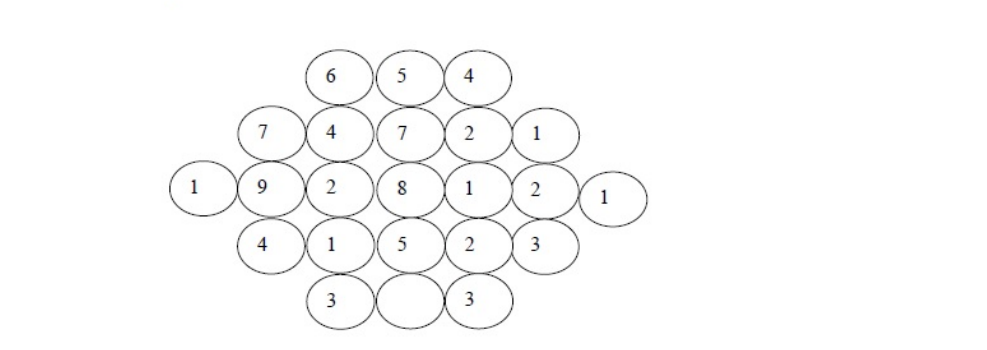
\includegraphics[width=0.65\columnwidth]{fig 1.png}
   \caption{}
   \label{fig:question65}
\end{figure}

A pharmaceutical company is contemplating the development of a vaccine against the most dangerous microbe. 
Which microbe should the company target in its first attempt?

\begin{multicols}{4}
  \begin{enumerate}
    \item P
    \item Q
    \item R
    \item S
  \end{enumerate}
\end{multicols} \hfill(GATE BT 2011)

\end{enumerate}
\end{document}